\documentclass[12pt,a4paper]{article}
\usepackage[spanish,es-tabla]{babel}
\usepackage{bbm}
\usepackage[utf8]{inputenc}
\usepackage{multicol}
\usepackage[T1]{fontenc}
\usepackage{graphicx}
\usepackage{gensymb}
\usepackage{amssymb, amsmath} %Paquetes matemáticos de la American Mathematical Society
\parskip=1 mm
\oddsidemargin -0.8 cm
\headsep -2 cm
\textwidth=17.8cm
\textheight=25.5cm
\begin{document}
\title{Laboratorio de Mecánica, Práctica 6 - Movimiento Rectilíneo Uniformemente Acelerado}
\date{18 de marzo del 2025}
\author{\textbf{Ortega Montero Fernando Naed} - Equipo 4\\
Yibran Morales Munguía\\
Victor Manuel Santillan Romero}
\maketitle
\section{Resumen} 

En este informe se trata el movimiento rectilíneo uniformemente acelerado (MRUA) con un riel de aire colocado con una inclinación suficiente para notar los efectos de la gravedad, haciendo uso de un cronometro para hacer las mediciones del móvil; parte de este informe se enfoca en el calculo de las incertidumbres combinadas, así como la propagación de incertidumbres sobre variables útiles para realizar una regresión lineal sobre los datos experimentales. 

\section{Introducción}

El movimiento rectilíneo uniformemente acelerado (MRUA) es un fenómeno físico que involucra la aceleración constante de un objeto a lo largo de una recta, donde la posición del objeto se conoce haciendo uso de la siguiente ecuación:

\[x(t) = x_0 + v_0 t + \frac{1}{2} a t^2\]

Donde…\\

$x(t)$ : Es la posición del objeto en el tiempo t, medida en (m).\\ 

$x_0$ : Es la posición inicial del objeto respecto del observador, medida en (m).\\

$V_0$ : Es la velocidad inicial del objeto, medida en ($\frac{m}{s}$).\\

$a$ : Es la aceleración del objeto, medida en ($\frac{m}{s^2}$).\\

$t$ : El tiempo, medido en (s).\\

Tomando a el observador en el mismo punto del cual el objeto inicia el movimiento, y tomando que el objeto parte del reposo, podemos decir que $x_0 = 0$ y $V_0 = 0$; con esto la ecuación no queda…

\[x(t) = \frac{1}{2} a t^2\]

Nótese que esta ecuación tiene a $t$ como un término cuadrático esto implica que la grafica se verá como una parábola, para poder hacer la regresión lineal será necesario hacer un cambio de variable que nos deje una ecuación de la posición con respecto del tiempo que tenga una variable lineal; para esto se usará $T = t^2$ dejándonos la ecuación de posición como:

\[x(T) = \frac{1}{2} a T\]

Como esta ecuación es lineal si se le puede aplicar regresión lineal, nótese que la pendiente de esta recta ideal será $\frac{a}{2}$. 

\section{Desarrollo experimental}

Para esta practica se utilizó un riel de aire, un carro para riel, una compresora de aire, un flexómetro (con una resolución de 0.1 cm), un cronometro (con una resolución de 0.01s) y masking tape.\\
Se colocaron diez marcas en el riel, haciendo uso masking tape con los intervalos de distancia expuestos en la Tabla 1, se coloco el riel de aire con suficiente inclinación para notar los efectos de la gravedad sobre el carro.\\
Con esto montado se coloco el carro en el riel en la posición inicial, y partiendo desde el reposo se soltó el carro, calculando el tiempo en el cual el carro alcanzó cada una de las maracas, con cinco mediciones por cada marca.  \\

\section{Resultados}

En la Tabla 1 se exponen las distancias consideradas, la media de los cinco tiempos tomados por cada marca, y la media del tiempo en cada marca al cuadrado (será utilizado para hacer el ajuste de la recta por regresión lineal).

\subsection{Calculo de la incertidumbre}

Para el cálculo de incertidumbre estándar combinada del tiempo se hará uso de la siguiente ecuación:

\[u_c(t) = \sqrt{u_A^2(t) + u_B^2(t)}\]

Donde…\\

$u_c(t)$ : Es la incertidumbre estándar combinada del tiempo.\\

$u_A(t)$ : Es la desviación estándar de la media de los tiempos medidos en cada marca. \\

$u_B(t)$ : Es la incertidumbre del cronometro (Su precisión).\\

Nótese que este cálculo se hizo para el promedio de los tiempos en cada marca, así mismo nótese que no se usara la precisión del cronometro como la incertidumbre tipo B, sino el promedio de los mínimos tiempos posibles medidos por uno de los experimentadores autores de este informe, este promedio fue 0.16 s, este tiempo será tomado como la incertidumbre tipo B.\\

De esto sigue la propagación de la incertidumbre para la variable $T = t^2$, usando la ley de la propagación de la incertidumbre tenemos la siguiente ecuación:

\[u^2_c (T) = \sum_{i = 1}^k \left( \frac{\partial T}{\partial x_i}\right) u^2(x_i)\]

Donde…\\

$u^2_c(T)$ : Es la incertidumbre de la variable T.\\

$x_i$ : Son las variables de las cuales depende la variable T; $T(x_1, x_2, …, x_k)$. Nótese que la variable T solo depende de t; $T(t) = t^2$, por lo que $x_i = t$.\\

$k$ : Son el número de variables de las cuales depende la variable T. Nótese que la variable T solo depende de t, por lo que $k = 1$.\\

$u^2(x_i)$ : Es la incertidumbre de cada variable de las cuales depende la variable T. Nótese que la variable T solo depende de t, por lo que $u^2(x_i) = u^2(t)$.\\

$\frac{\partial T}{\partial x_i}$: Es la derivada parcial de cada variable de las cuales depende la variable T. Nótese que la variable T solo depende de t, por lo que $\frac{\partial T}{\partial x_i} = \frac{d T}{d x_i} = 2t$.\\

Finalmente, esta ecuación nos queda:

\[u^2_c (T) = \sum_{i = 1}^1 \left( \frac{\partial T}{\partial t}\right)^2 u^2(t)\]
\[u^2_c (T) = (2t)^2 u^2(t)\]
\[u_c (T) = 2t u(t)\]

Nótese que este calculo se hizo para cada T, o mejor dicho para cada cuadrado del promedio de los tiempos en cada marca. 


\begin{table}[h!]
\begin{center}
\begin{tabular}{|c|c|c|c|}
\hline
No. & s (m) & t (s) & $T = t^2$ ($s^2$)\\
\hline
1 & 5.20 (0.1) cm & 0.70 (0.16) s & 0.49 (0.22) $s^2$ \\ \hline
2 & 17.7 (0.1) cm & 1.49 (0.16) s & 2.22 (0.48) $s^2$ \\ \hline
3 & 30.2 (0.1) cm & 2.00 (0.17) s & 4.00 (0.68) $s^2$ \\ \hline
4 & 42.7 (0.1) cm & 2.22 (0.16) s & 4.93 (0.71) $s^2$ \\ \hline
5 & 55.2 (0.1) cm & 2.58 (0.16) s & 6.66 (0.83) $s^2$ \\ \hline
6 & 67.7 (0.1) cm & 2.91 (0.16) s & 8.47 (0.93) $s^2$ \\ \hline
7 & 80.2 (0.1) cm & 3.13 (0.17) s & 9.80 (1.06) $s^2$ \\ \hline
8 & 92.7 (0.1) cm & 3.36 (0.16) s & 11.29 (1.08) $s^2$ \\ \hline
9 & 105.2 (0.1) cm & 3.44 (0.17) s & 11.83 (1.17) $s^2$ \\ \hline
10 & 117.7 (0.1) cm & 3.68 (0.17) s & 13.54 (1.25) $s^2$ \\ \hline
\end{tabular}
\caption{Tiempos medidos de un movimiento acelerado. }
\end{center}
\end{table}

\begin{figure}[h!]
\centering
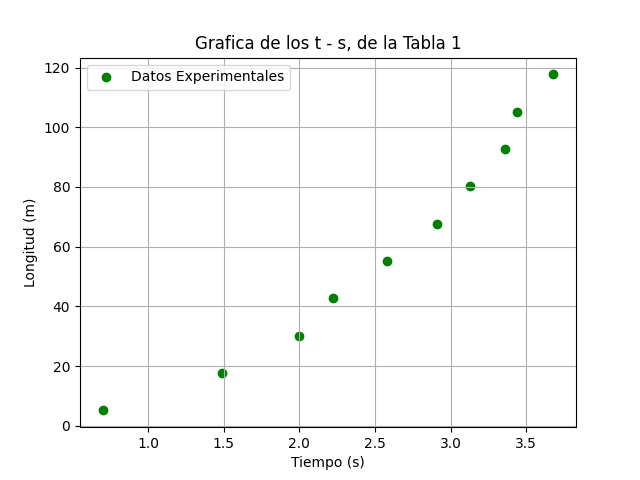
\includegraphics[scale=0.68]{t-s.png}
\end{figure}

\begin{figure}[h!]
\centering
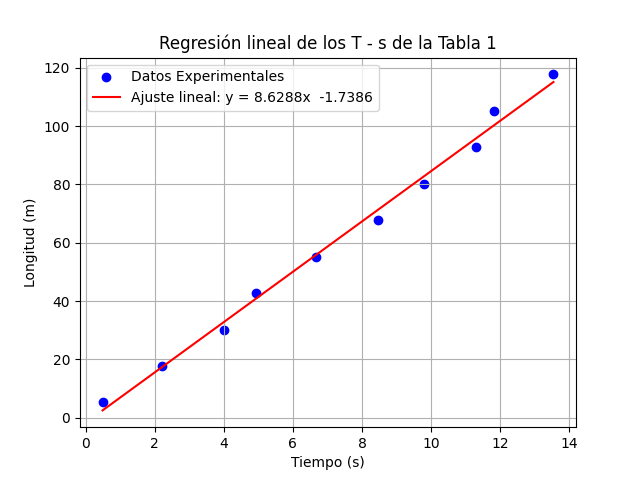
\includegraphics[scale=0.68]{2T-s.png}
\end{figure}

\newpage

\section{Discusión}

Gráfica de los t-s, de la Tabla 1 se puede notar que los datos siguen una parábola, esto sigue el planteamiento teórico expuesto en la Introducción donde se plantea una ecuación de segundo grado. \\
Así mismo después del cambio de variable de $T = t^2$ en la Tabla 1, los datos se comportaron como una recta lo cual sigue el planteamiento teórico expuesto en la Introducción, donde después del cambio de variable se consigue una ecuación de primer grado, con la pendiente de esta recta como la aceleración.\\

\section{Conclusión}

Esta practica es un perfecto ejemplo para la obtención de incertidumbres, tanto de tipo A y B como la incertidumbre combinada, el análisis de la correcta incertidumbre de los instrumentos; como lo fue la incertidumbre del cronometro, así como un ejemplo sencillo del uso de la ley de propagación de incertidumbres; cuando se realizo el cambio de variable de $T = t^2$.\\
Esta práctica es útil para ejemplificar el uso de una herramienta útil como lo es el cambio de variable para adaptar una ecuación de grado superior a una ecuación de primer grado a la cual se le puede aplicar regresión lineal. \\
Finalmente se recomienda el uso de foto compuertas para la realización de este experimento, por su sencillez y su precisión a la hora de medir sobre el cronometro.

\section{Referencias}

Miranda, Javier. (2025) \textit{Física Experimental. Introducción a los conceptos y métodos.} Recuperado el 18, 03, 2025, de https://copitarxives.fisica.unam.mx/LT0006ES/LT0006ES.pdf \\

Miranda, Javier. (2000). \textit{EVALUACIÓN DE LA INCERTIDUMBRE EN DATOS EXPERIMENTALES.} \\

Pérez, Héctor. (2018). \textit{Física general.}(Sexta Edición.). México: PATRIA educación \\





\end{document}